\chapter{Przegląd strategii czasu rzeczywistego}

“Starożytni świat widzieli inaczej, mniej płasko”\cite{gbobrektvgry}. Dobrze obrazującym ówczesne postrzeganie przestrzeni przykładem jest mapa Imperium Rzymskiego,
pokazana na \ref{fig:mapaIR}. Czytanie jej dosłownie mija się z celem. Nie są na niej zachowane ani proporcje, ani strony świata. Mimo tego, że
basen Morza Śródziemnego został ówcześnie dosyć dokładnie oddany, “nie wydaje się, aby Rzymianom współczesna kartograficzna wierność była potrzebna”\cite{gbobrektvgry}.
“Dowódcy opierali się na swojej wiedzy, wiedzy wynajętych przewodników oraz informacjach zwiadowców i tubylców”\cite{gbobrektvgry}.
\begin{figure}[htbp]
    \centering
    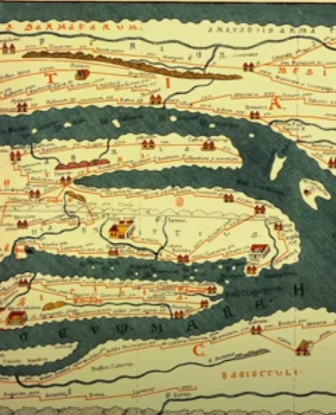
\includegraphics[width=0.5\textwidth]{images/mapaIR.png}
    \caption{Mapa basenu Morza Śródziemnego z czasów Imperium Rzymskiego}\label{fig:mapaIR}
\end{figure}

Na odbiór gry wpływają zawarte w niej mechaniki. Twórcy bardzo częstostosują w nich uproszczenia, co ma na celu
ułatwienie graczowi wykonywanie zadań. Ma to jednak ogromny wpływ na zachowanie realizmu w grach, zwłaszcza tych opartych
na wydarzeniach historycznych oraz prawdziwym świecie. 

W niniejszym rozdziale zostały przedstawione wybrane mechaniki wykorzystywane w grach typu RTS. Omówione zostało ich
działanie na podstawie przykładów z najpopularniejszych gier. Celem tego jest obrazowe zaprezentowanie ich integralności
w grach oraz wpływu na rozgrywkę.